\documentclass{article}

\usepackage{tikz}
\usepackage{ifthen}
\usepackage{caption}
\usepackage{subfig}

\usetikzlibrary{calc,positioning,shadows.blur,decorations.pathreplacing}
\usepackage{etoolbox}

\definecolor{r0d}{RGB}{255,214,226}
\definecolor{r1d}{RGB}{165,201,239}
\definecolor{r2d}{RGB}{196,228,239}

\tikzset{%
  brace/.style = { decorate, decoration={brace, amplitude=5pt} },
  mbrace/.style = { decorate, decoration={brace, amplitude=5pt, mirror} },
  label/.style = { black, midway, scale=0.5, align=center },
  toplabel/.style = { label, above=.5em, anchor=south },
  leftlabel/.style = { label,rotate=90,left=1.9em,anchor=north },   
  rightlabel/.style = { label,rotate=-90,right=1.5em,anchor=north },   
  bottomlabel/.style = { label, below=.5em, anchor=north },
  force/.style = { rotate=-90,scale=0.4 },
  round/.style = { rounded corners=2mm },
  legend/.style = { right,scale=0.4 },
  nosep/.style = { inner sep=0pt },
  generation/.style = { anchor=base }
}


\begin{document}

\title{Sparse Matrix-Vector Multiplication with CUDA}
\author{Georgii Evtushenko}

\maketitle

\section{Introduction}

Standard methods of differential equations discretization usually lead to systems of linear equations. 
A general feature of produced systems is that the number of entries in each equation depends on local topological features of the discretization.
Thus, the matrices generated by these systems contain a lot of zeroes (image \ref{fem_to_sparse_matrix}). It's possible to take advantage of knowledge about zeroes' position by 
storing matrices in special data structures.The abstract data type for these structures is called the sparse matrix. 
This post provides an efficiency review for basic sparse matrix data structures in context of sparse matrix vector multiplication (SpMV) on GPU.

\begin{figure}
  \centering
  \subfloat[Mesh]
  {
    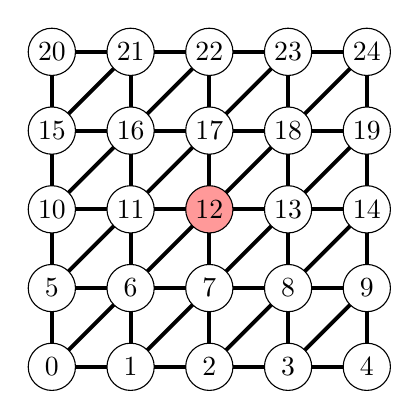
\begin{tikzpicture}[circ/.style = {circle, draw, inner sep=0pt, minimum size=3pt, outer sep=0pt, minimum size=6mm}]
      \pgfmathsetmacro{\lastelementsinrow}{4}
      \foreach \x in {0,...,\lastelementsinrow}
      {
        \foreach \y in {0,...,\lastelementsinrow}
        {
          \pgfmathtruncatemacro{\label}{\y * \lastelementsinrow + \y + \x}
          \ifthenelse{\x=2 \AND \y=2}{\node (\x\y) [circ,fill=red!40] at (\x, \y) {\label}}{\node (\x\y) [circ] at (\x, \y) {\label}};
        }
      }

      \foreach \x in {1,...,\lastelementsinrow}
      {
        \foreach \y in {0,...,\lastelementsinrow}
        {
          \pgfmathtruncatemacro{\px}{\x - 1}
          \draw [line width=0.5mm] (\x\y) -- (\px\y);
        }
      }

      \foreach \x in {0,...,\lastelementsinrow}
      {
        \foreach \y in {1,...,\lastelementsinrow}
        {
          \pgfmathtruncatemacro{\py}{\y - 1}
          \draw [line width=0.5mm] (\x\y) -- (\x\py);
        }
      }

      \foreach \x in {1,...,\lastelementsinrow}
      {
        \foreach \y in {1,...,\lastelementsinrow}
        {
          \pgfmathtruncatemacro{\py}{\y - 1}
          \pgfmathtruncatemacro{\px}{\x - 1}
          \draw [line width=0.5mm] (\x\y) -- (\px\py);
        }
      }
    \end{tikzpicture}
  }
  \qquad
  \subfloat[Matrix]
  {
    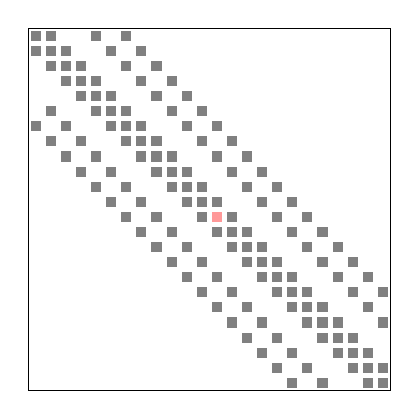
\begin{tikzpicture}
      \pgfmathsetmacro{\size}{4.6}
      \pgfmathsetmacro{\es}{\size/24}
      \pgfmathsetmacro{\pd}{\es/6}
      \pgfmathsetmacro{\ebs}{\es - 2 * \pd}
      \draw (0,0) rectangle ++(\size,\size);

      % Diagonal part
      \foreach \x in {0,...,23}
        \foreach \y in {0,...,23}
         \ifthenelse{\x=\y}
         {
           \ifthenelse{\y=12}
           {
             \fill [red!40] (\es * \x + \pd, \size - \es * \y - \es + \pd) rectangle ++(\ebs, \ebs)
           }
           {
             \fill [gray] (\es * \x + \pd, \size - \es * \y - \es + \pd) rectangle ++(\ebs, \ebs)
           }
         }{};

      % Left part
      \foreach \y in {1,...,23}
       \fill [gray] (\es * \y - \es + \pd, \size - \es * \y - \es + \pd) rectangle ++(\ebs, \ebs);

      % Right part
      \foreach \y in {0,...,22}
       \fill [gray] (\es * \y + \es + \pd, \size - \es * \y - \es + \pd) rectangle ++(\ebs, \ebs);

      % Bottom part
      \foreach \y in {5,...,23}
       \fill [gray] (\es * \y - 4 * \es + \pd, \size - \es * \y - \es + \pd) rectangle ++(\ebs, \ebs);

      % Top part
      \foreach \y in {0,...,19}
       \fill [gray] (\es * \y + 4 * \es + \pd, \size - \es * \y - \es + \pd) rectangle ++(\ebs, \ebs);

      % Diag part
      \foreach \y in {0,...,17}
       \fill [gray] (\es * \y + 6 * \es + \pd, \size - \es * \y - \es + \pd) rectangle ++(\ebs, \ebs);
      \foreach \y in {6,...,23}
       \fill [gray] (\es * \y - 6 * \es + \pd, \size - \es * \y - \es + \pd) rectangle ++(\ebs, \ebs);
    \end{tikzpicture}
  }
  \caption{A simple finite element mesh model}
  \label{fem_to_sparse_matrix}
\end{figure}

\section{Data Structures for Sparse Matrices}
In general, SpMV is limited by memory bandwidth. The storage format used for the sparse matrix defines SpMV algorithm. Each of this
algorithms has it's own granularity, which impacts performance. The primary distinction among sparse matrix representations is the 
sparsity pattern, or the structure of the nonzero entries, for which they are best suited. 

\subsection{CSR}

The \textit{Compressed Sparse Row} (CSR) format is a general sparse matrix format. CSR format consists of three arrays: \textit{row\_ptr},
non-zeroes' \textit{columns} and matrix \textit{values}. The row's non-zero values are stored consequentially in \textit{values} array. The \textit{row\_ptr} array
is used to divide \textit{values} array into separate rows. It's size is equal to $n\_rows + 1$. For each non-zero value column index is stored in 
\textit{columns} array.

\begin{figure}
  \centering
  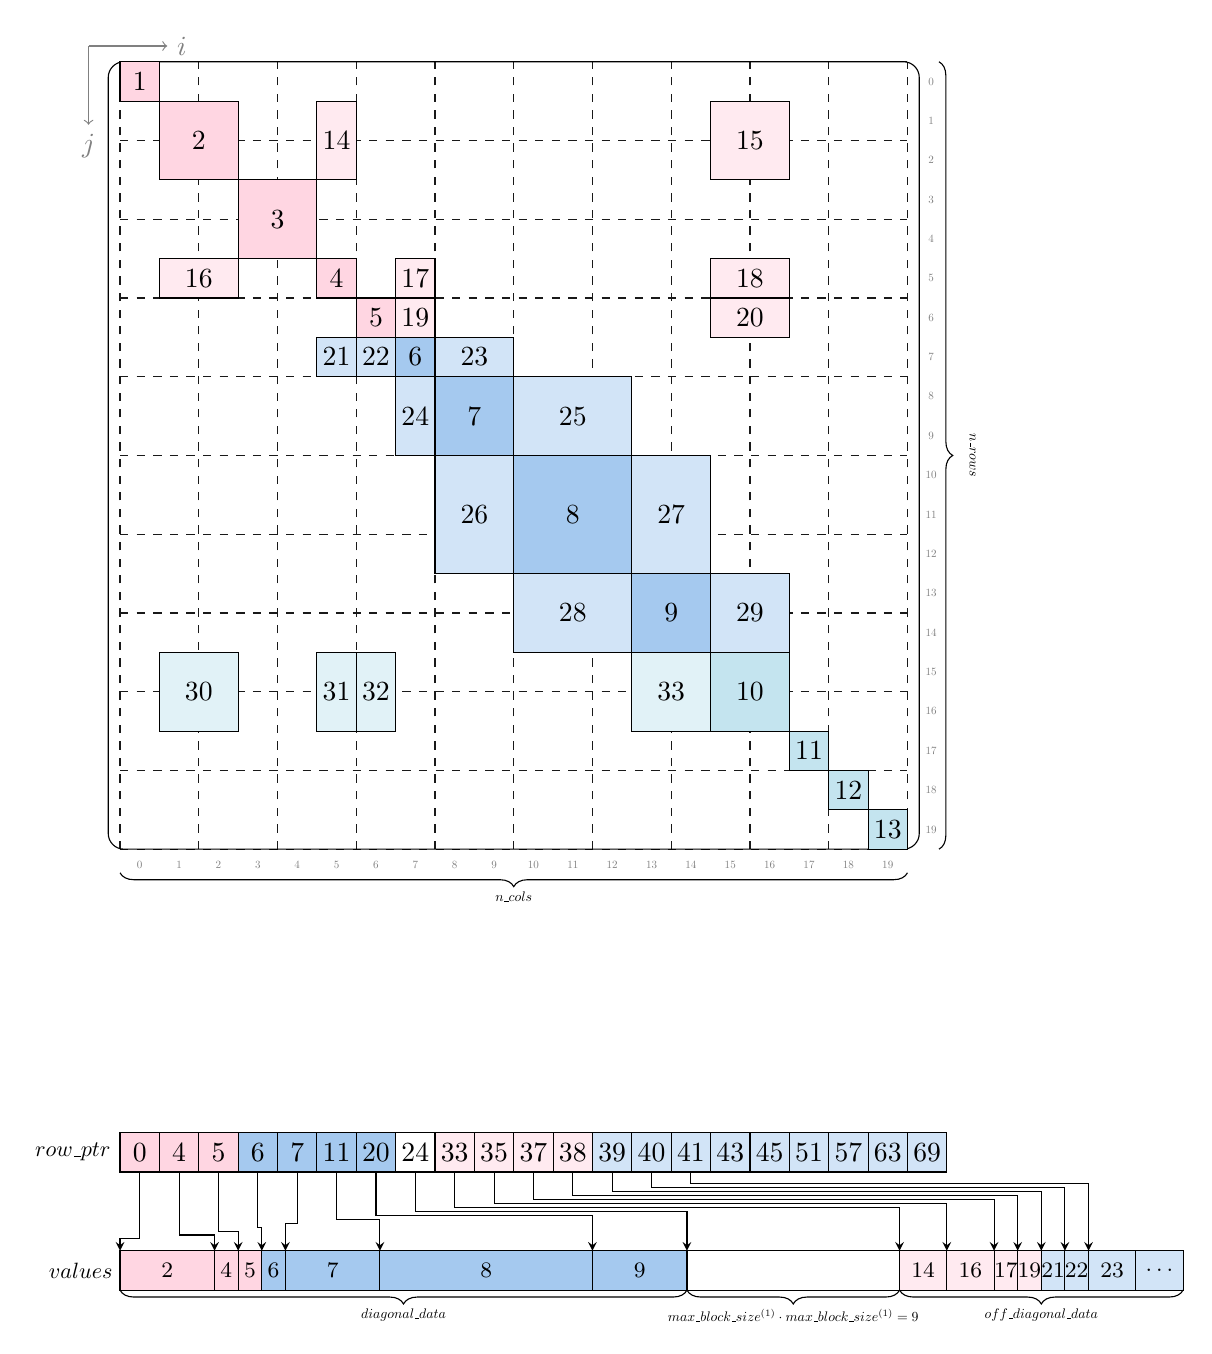
\begin{tikzpicture}[circ/.style = {circle, draw, inner sep=0pt, minimum size=3pt, outer sep=0pt, minimum size=6mm}]

  \foreach \y in {0,...,19} {
    \node[scale=0.4,text=gray] at (10.3,10.0 - 0.5*\y - 0.25) {\y};
  }

  \foreach \x in {0,...,19} {
    \node[scale=0.4,text=gray] at (0.5*\x + 0.25,-0.2) {\x};
  }

  \draw[->,gray] (-0.4,10.2) -- (0.6,10.2) node[right] {$i$};
  \draw[->,gray] (-0.4,10.2) -- (-0.4,9.2) node[below] {$j$};

  % Elements mesh
  \draw[step=1.0,black!90!white,thin,dashed,line width=0.4] (0.0,0.0) grid (10.0,10.0);

  \draw[round] (-0.15,0) rectangle (10.15,10);

  % Right braces
  \draw [mbrace] (10.4,0.0)  -- (10.4,10.0) node[rightlabel] {$n\_rows$};

  % Bottom braces
  \draw [mbrace] (0.0,-0.3) -- (10,-0.3) node[bottomlabel] {$n\_cols$};


  % RANK 0
  \draw[fill=r0d] (0,9.5) rectangle (0.5,10) node[pos=.5] {1}; % DIAG
  \draw[fill=r0d] (0.5,8.5) rectangle (1.5,9.5) node[pos=.5] {2}; 
  \draw[fill=r0d] (1.5,7.5) rectangle (2.5,8.5) node[pos=.5] {3}; 
  \draw[fill=r0d] (3.0,7.0) rectangle (2.5,7.5) node[pos=.5] {4}; 
  \draw[fill=r0d] (3.5,6.5) rectangle (3.0,7.0) node[pos=.5] {5}; 

  \draw[fill=r0d!50!white] (2.5,8.5) rectangle (3.0,9.5) node[pos=.5] {14}; % OFF-DIAG
  \draw[fill=r0d!50!white] (7.5,8.5) rectangle (8.5,9.5) node[pos=.5] {15}; 
  \draw[fill=r0d!50!white] (0.5,7.0) rectangle (1.5,7.5) node[pos=.5] {16}; 
  \draw[fill=r0d!50!white] (3.5,7.0) rectangle (4.0,7.5) node[pos=.5] {17}; 
  \draw[fill=r0d!50!white] (7.5,7.0) rectangle (8.5,7.5) node[pos=.5] {18}; 
  \draw[fill=r0d!50!white] (3.5,6.5) rectangle (4.0,7.0) node[pos=.5] {19}; 
  \draw[fill=r0d!50!white] (7.5,6.5) rectangle (8.5,7.0) node[pos=.5] {20}; 

  $$% RANK 1
  \draw[fill=r1d] (4.0,6.0) rectangle (3.5,6.5) node[pos=.5] {6}; % DIAG
  \draw[fill=r1d] (4.0,6.0) rectangle (5.0,5.0) node[pos=.5] {7}; 
  \draw[fill=r1d] (5.0,5.0) rectangle (6.5,3.5) node[pos=.5] {8}; 
  \draw[fill=r1d] (6.5,3.5) rectangle (7.5,2.5) node[pos=.5] {9}; 

  \draw[fill=r1d!50!white] (3.0,6.0) rectangle (2.5,6.5) node[pos=.5] {21}; % OFF-DIAG
  \draw[fill=r1d!50!white] (3.0,6.0) rectangle (3.5,6.5) node[pos=.5] {22}; 
  \draw[fill=r1d!50!white] (4.0,6.0) rectangle (5.0,6.5) node[pos=.5] {23}; 
  \draw[fill=r1d!50!white] (3.5,6.0) rectangle (4.0,5.0) node[pos=.5] {24}; 
  \draw[fill=r1d!50!white] (5.0,6.0) rectangle (6.5,5.0) node[pos=.5] {25}; 
  \draw[fill=r1d!50!white] (4.0,5.0) rectangle (5.0,3.5) node[pos=.5] {26}; 
  \draw[fill=r1d!50!white] (6.5,5.0) rectangle (7.5,3.5) node[pos=.5] {27}; 
  \draw[fill=r1d!50!white] (5.0,3.5) rectangle (6.5,2.5) node[pos=.5] {28}; 
  \draw[fill=r1d!50!white] (7.5,3.5) rectangle (8.5,2.5) node[pos=.5] {29}; 


  % RANK 2
  \draw[fill=r2d] (7.5,2.5) rectangle (8.5,1.5)  node[pos=.5] {10}; 
  \draw[fill=r2d] (8.5,1.5) rectangle (9.0,1.0)  node[pos=.5] {11}; 
  \draw[fill=r2d] (9.0,1.0) rectangle (9.5,0.5)  node[pos=.5] {12}; 
  \draw[fill=r2d] (9.5,0.5) rectangle (10,0)     node[pos=.5] {13}; 

  \draw[fill=r2d!50!white] (0.5,2.5) rectangle (1.5,1.5) node[pos=.5] {30}; 
  \draw[fill=r2d!50!white] (2.5,2.5) rectangle (3.0,1.5) node[pos=.5] {31}; 
  \draw[fill=r2d!50!white] (3.0,2.5) rectangle (3.5,1.5) node[pos=.5] {32}; 
  \draw[fill=r2d!50!white] (6.5,2.5) rectangle (7.5,1.5) node[pos=.5] {33}; 


  % RHS
  \edef\lasty{0}
  \edef\ynum{1}

  % =====================================================
  % ================== Data structures ================== 
  % =====================================================

  % RHS OFFSETS
  \edef\ybot{-2.0}
  \edef\cheight{0.5}

  \edef\xnum{0}
  \edef\lastblockoffset{0}
  \edef\lastyoffset{\ybot-\cheight*0.8}

  % ROWS NON ZEROS
  \pgfmathparse{\ybot-\cheight*2.2}
  \xdef\ybot{\pgfmathresult}

  \edef\xnum{0}
  \edef\lastblockoffset{0}
  \edef\lastyoffset{\ybot-\cheight*0.8}

  % MATRIX OFFSETS
  \pgfmathparse{\ybot-\cheight*2}
  \xdef\ybot{\pgfmathresult}
  \edef\cwidth{0.3}

  \node[scale=0.8] at (-0.6,\ybot+\cheight/2) {$row\_ptr$};

  \edef\xnum{0}
  \edef\lastblockoffset{0}
  \edef\lastyoffset{\ybot-\cheight*1.8}

  \foreach \offset in {0,4,5,6,7,11,20,24,33,35,37,38,39,40,41,43,45,51,57,63,69} {
    \pgfmathparse{\cwidth*\offset}
    \xdef\lastblockoffset{\pgfmathresult}

    \pgfmathparse{\lastyoffset+\cheight/10}
    \xdef\lastyoffset{\pgfmathresult}

    \ifthenelse{\xnum<3}
    { \draw[fill=r0d] (\xnum*0.5,\ybot) rectangle (\xnum*0.5+0.5,\ybot+\cheight) node[pos=.5] {\offset}; }
    {
      \ifthenelse{\xnum<7}
      { \draw[fill=r1d] (\xnum*0.5,\ybot) rectangle (\xnum*0.5+0.5,\ybot+\cheight) node[pos=.5] {\offset}; }
      {
        \ifthenelse{\xnum<8}
        { \draw[fill=white] (\xnum*0.5,\ybot) rectangle (\xnum*0.5+0.5,\ybot+\cheight) node[pos=.5] {\offset}; }
        {
          \ifthenelse{\xnum<12}
          { \draw[fill=r0d!50!white] (\xnum*0.5,\ybot) rectangle (\xnum*0.5+0.5,\ybot+\cheight) node[pos=.5] {\offset}; }
          { 
            \ifthenelse{\xnum<22}
            { \draw[fill=r1d!50!white] (\xnum*0.5,\ybot) rectangle (\xnum*0.5+0.5,\ybot+\cheight) node[pos=.5] {\offset}; }
            { \draw[fill=white] (\xnum*0.5,\ybot) rectangle (\xnum*0.5+0.5,\ybot+\cheight) node[pos=.5] {\offset}; }
          }
        }
      }
    }

    \ifthenelse{\xnum<15}
    { \draw[>=stealth,->] (\xnum*0.5+\cheight/2,\ybot) |- (\lastblockoffset,\lastyoffset) -| (\lastblockoffset,\ybot-2*\cheight); }
    { }

    \pgfmathparse{int(\xnum+1)}
    \xdef\xnum{\pgfmathresult}
  }

  % MATRIX DATA
  \pgfmathparse{\ybot-\cheight*3}
  \xdef\ybot{\pgfmathresult}

  \node[scale=0.8] at (-0.5,\ybot+\cheight/2) {$values$};

  % Diagonal
  \draw[fill=r0d]  (0* \cwidth,\ybot) rectangle (4* \cwidth,\ybot+\cheight) node[pos=0.5] {\footnotesize 2};
  \draw[fill=r0d]  (4* \cwidth,\ybot) rectangle (5* \cwidth,\ybot+\cheight) node[pos=0.5] {\footnotesize 4};
  \draw[fill=r0d]  (5* \cwidth,\ybot) rectangle (6* \cwidth,\ybot+\cheight) node[pos=0.5] {\footnotesize 5};
  \draw[fill=r1d]  (6* \cwidth,\ybot) rectangle (7* \cwidth,\ybot+\cheight) node[pos=0.5] {\footnotesize 6};
  \draw[fill=r1d]  (7* \cwidth,\ybot) rectangle (11*\cwidth,\ybot+\cheight) node[pos=0.5] {\footnotesize 7};
  \draw[fill=r1d]  (11*\cwidth,\ybot) rectangle (20*\cwidth,\ybot+\cheight) node[pos=0.5] {\footnotesize 8};
  \draw[fill=r1d]  (20*\cwidth,\ybot) rectangle (24*\cwidth,\ybot+\cheight) node[pos=0.5] {\footnotesize 9};
  \draw[fill=white](24*\cwidth,\ybot) rectangle (33*\cwidth,\ybot+\cheight) node[pos=0.5] {};
  % Off-Diagonal
  \draw[fill=r0d!50!white] (33*\cwidth,\ybot) rectangle (35*\cwidth,\ybot+\cheight) node[pos=0.5] {\footnotesize 14};
  \draw[fill=r0d!50!white] (35*\cwidth,\ybot) rectangle (37*\cwidth,\ybot+\cheight) node[pos=0.5] {\footnotesize 16};
  \draw[fill=r0d!50!white] (37*\cwidth,\ybot) rectangle (38*\cwidth,\ybot+\cheight) node[pos=0.5] {\footnotesize 17};
  \draw[fill=r0d!50!white] (38*\cwidth,\ybot) rectangle (39*\cwidth,\ybot+\cheight) node[pos=0.5] {\footnotesize 19};
  \draw[fill=r1d!50!white] (39*\cwidth,\ybot) rectangle (40*\cwidth,\ybot+\cheight) node[pos=0.5] {\footnotesize 21};
  \draw[fill=r1d!50!white] (40*\cwidth,\ybot) rectangle (41*\cwidth,\ybot+\cheight) node[pos=0.5] {\footnotesize 22};
  \draw[fill=r1d!50!white] (41*\cwidth,\ybot) rectangle (43*\cwidth,\ybot+\cheight) node[pos=0.5] {\footnotesize 23};
  \draw[fill=r1d!50!white] (43*\cwidth,\ybot) rectangle (45*\cwidth,\ybot+\cheight) node[pos=0.5] {\footnotesize $\dots$};

  \draw [mbrace] (0 *\cwidth,\ybot)  -- (24*\cwidth,\ybot) node[bottomlabel] {$diagonal\_data$};
  \draw [mbrace] (24*\cwidth,\ybot)  -- (33*\cwidth,\ybot) node[bottomlabel] {$max\_block\_size^{(1)} \cdot max\_block\_size^{(1)}=9$};
  \draw [mbrace] (33*\cwidth,\ybot)  -- (45*\cwidth,\ybot) node[bottomlabel] {$off\_diagonal\_data$};
  \end{tikzpicture}
  \caption{Example of Compressed Sparse Row (CSR) matrix format}
  \label{csr_format}
\end{figure}

General CSR SpMV implementation works at the granularity of threads per row. This implementation is usually referenced as CSR-Scalar.

\subsection{COO}

\subsection{ELL}

\subsection{Hybrid}


\section{Conclusion}
Write your conclusion here.

\end{document}
